\section{Parametriset käyrät ja pinnat} \label{parametriset käyrät}
\alku
\index{funktio A!f@parametrinen käyrä ja pinta|vahv}
\index{parametrinen käyrä|vahv}
\index{parametri(sointi)!c@käyrän|vahv}
\index{kzyyrzy@käyrä|vahv}

Tason tai avaruuden \kor{parametriseksi käyräksi} sanotaan \pain{funktiota} muotoa
\[ 
t \in A\ \map\ P(t)\in E^d, 
\]
missä $A \subset \R$ on \pain{väli} (usein suljettu väli) ja $d=2$ tai $d=3$. Muuttujaa $t$ 
sanotaan tässä \kor{parametriksi}. Käyrä on \kor{tasokäyrä} jos $d=2$, \kor{avaruuskäyrä} jos 
$d=3$. Käyttäen jo tutuksi tulleita geometrisia vastaavuuksia voidaan kirjoittaa
\[
P(t)\ \vastaa\ \Vect{OP}(t)\ 
                = \left\{ \begin{array}{lrlll} 
                   x(t)\vec{i}+y(t)\vec{j} & \vastaa & (x(t),y(t)),      & & (d=2) \\
                   x(t)\vec{i}+y(t)\vec{j}+z(t)\vec{k} & \vastaa & (x(t),y(t),z(t)), & & (d=3)
                          \end{array} \right.
\]
missä $x,y,z$ ovat funktioita tyyppiä $f: A \kohti \R$. Tämän mukaisesti parametrinen käyrä 
\index{vektoric@vektoriarvoinen funktio}%
voidaan tulkita reaalimuuttujan \kor{vektoriarvoiseksi} funktioksi, jolloin luonteva esitystapa
on myös vektorimerkintä
\[ 
\vec{r}\,(t)\ =\ \begin{cases} 
   x(t)\vec{i}+y(t)\vec{j},\ \ t \in A,                   &\text{(tasokäyrä)} \\
   x(t)\vec{i}+y(t)\vec{j}+z(t)\vec{k},\ \ t \in A. \quad &\text{(avaruuskäyrä)}
               \end{cases}
\]
Liittyen vastaavuuteen $\mathit{E^d} \vast \R^d$ voidaan parametrinen käyrä esittää yhtä hyvin 
yhtälöryhmänä, esim.\ tasokäyrän tapauksessa
\[ 
(x,y)\ =\ (x(t),y(t)) \qekv 
        \begin{cases} \,x = x(t), \\ \,y = y(t). \end{cases} \quad 
\text{(tasokäyrä)}\footnote[2]{Merkinnöissä $x=x(t)$ ja $y=y(t)$ on symboleja $x,y$ käytetty
kahdessa eri merkityksessä: oikealla funktion, vasemmalla ko.\ funktion arvojoukon alkion
symbolina. Tämän tyyppisiä epäloogisuuksia pidetään matematiikan käytännössä siedettävinä,
syystä että ne yksinkertaistavat merkintöjä.}
\]
\begin{Exa} Reaalimuuttujan funktio $f: [a,b] \kohti \R$ voidaan tulkita parametriseksi
tasokäyräksi
\[ 
\vec{r} = \vec{r}\,(t) = t\vec{i} + f(t)\vec{j} \qekv 
                           \begin{cases} \,x = x(t) = t, \\ \,y = y(t) = f(t),\ \ t \in [a,b]. 
                           \end{cases} \loppu 
\] 
\end{Exa}
\begin{Exa} Luvuista \ref{suorat ja tasot} ja \ref{koordinaatistot} tuttuja parametrisia 
avaruuskäyriä ovat
\begin{align*}
&\text{avaruussuora:}\quad \vec{r}\,(t)\ 
          =\ (x_0 + \alpha t)\vec{i} + (y_0 + \beta t)\vec{j} + (z_0 + \gamma t)\vec{k}\ 
          =\ \vec{r}_0 + t \vec{v}, \quad t \in \R, \\ 
&\text{ruuviviiva:}\quad \begin{cases}
                          \,x = x(\varphi) = R\cos\varphi, \\ 
                          \,y = y(\varphi) = R\sin\varphi, \\ 
                          \,z = z(\varphi) = a\varphi,\ \ \varphi \in \R. \loppu
                         \end{cases} 
\end{align*} 
\end{Exa}
Parametrisen käyrän euklidiseen avaruuteen jättämä 'geometrinen jälki' on arvojoukko 
$S = \{P(t) \vastaa \vec{r}\,(t) \mid t \in A\} \subset E^d$, johon voidaan viitata sellaisilla 
termeillä kuin \kor{käyrä} (engl.\ curve) tai (käyrän) \kor{kaari} (engl.\ arc). 
Yksinkertaisimmillaan $S$ on jostakin pisteestä $A$ alkava ja toiseen pisteeseen $B$ päättyvä,
\index{yksinkertainen!c@käyrä, kaari} \index{kaari (käyrän)}%
itseään leikkaamaton ja yhtenäinen viiva, eli nk.\ \kor{yksinkertainen kaari} (engl.\ 
simple arc). Tällaisia ovat esim.\ jana tai ympyrän kaari. Viiva voi myös olla päättymätön, 
kuten suora, tai umpinainen
\index{suljettu käyrä}%
\kor{suljettu käyrä} (engl.\ closed curve), kuten tason tai 
avaruuden ympyräviiva. Joukko $S$ voi myös olla itseään leikkaava, eli siinä voi olla 
'silmukoita'.\footnote[2]{Muodossa $S = \{P(t) \vastaa \vec{r}\,(t) \mid t \in A\}$
määriteltyjen taso- tai avaruuskäyrien geometrista luokittelua ei todellisuudessa voi
täsmentää ilman funktion $\vec{r}$ koordinaattifunktioile $x,y,z$ asetettavia lisäehtoja.
Vrt.\ käyriä koskeva alaviite edellisessä luvussa.}
Jos lähtökohdaksi otetaan vain tällainen 'viiva' $S$, eli pelkästään geometrinen objekti, niin 
funktiota $\vec{r}\,(t),\ t \in A$, jonka arvojoukko $=S$, sanotaan $S$:n 
\kor{parametriesitykseksi} eli \kor{parametrisoinniksi} (parametrisaatioksi). 
Parametrisoivan funktion $t \in A \map \vec{r}\,(t) \in S$ ei tarvitse olla injektiivinen, ts.\ 
samaan pisteeseen $P \in S$ voidaan päätyä monella (jopa äärettömän monella) parametrin
arvolla.
\begin{Exa} \label{ympyrän parametrisaatio} Tason ympyräviivan 
\[ 
S = \{P \vastaa (x,y) \in \R^2 \mid (x-x_0)^2 + (y-y_0)^2 = R^2\} 
\]
luonteva parametrisointi on
\[ 
\begin{cases} x = x_0 + R \cos t, \\ y = y_0 + R\,\sin t,\ \ t \in [0,2\pi). \end{cases} 
\]
Tässä voi välin $[0,2\pi)$ tilalla olla myös esim.\ $A = (-\pi,\pi]$, $A = [0,2\pi]$ tai
$A = \R$. Kahdessa jälkimmäisessä vaihtoehdossa parametrisointi ei ole injektio. \loppu
\end{Exa}
\begin{Exa} Jos $S$ on avaruussuora, niin tämän tavanomaisin parametrisaatio on 
$\vec{r}\,(t) = \vec{r}_0 + t \vec{v},\ t \in \R$, missä $P_0 \vastaa \vec{r}_0$ on suoran
piste ja $\vec{v} \neq \vec{0}$ suoran suuntavektori (vrt.\ Luku \ref{suorat ja tasot}).
Tällaisiakin parametrisointeja on jo äärettömän monta, mutta mahdollisuudet eivät lopu tähän:
Jos $\vec{r}_0$ ja $\vec{v}$ täyttävät mainitut ehdot, niin parametrisoinniksi voidaan
yleisemmin valita
\[ 
\vec{r}\,(t)\ =\ \vec{r}_0 + f(t)\,\vec{v}, \quad t \in A, 
\]
missä funktion $f: A \kohti \R$ valintaa rajoittaa vain ehto $\RF_f = \R$. Esimerkiksi voidaan 
valita $f(t) = \tan t,\ A = (-\pi/2,\pi/2)$ ($f$ injektio), tai $f(t) = t \sin t,\ A = \R$ 
($f$ ei injektio).  \loppu \end{Exa}
\jatko \begin{Exa} (jatko) Jos halutaan parametrisoida suoralla $S$ oleva jana, jonka 
päätepisteet ovat $A \vastaa \vec{r}_1$ ja $B \vastaa \vec{r}_2$, niin tämä käy muodossa
\[ 
\vec{r}\,(t) = f(t)\,\vec{r}_1 + [1-f(t)]\,\vec{r}_2,\ \ t \in A, 
\]
missä $f$ on funktio tyyppiä $f: A \kohti \R,\ A \subset \R$, ja $\RF_f = [0,1]$.
Yksinkertaisin parametrisointi saadaan, kun valitaan $A = [0,1]$ ja $f(t) = t$. \loppu 
\end{Exa}
Jos tasokäyrän yhtälöistä $x = x(t),\ y = y(t),\ t \in A$ pystytään eliminoimaan parametri
$t$, on tuloksena yhtälö muotoa
\[ 
F(x,y) = 0, 
\]
missä siis $F$ on kahden muuttujan funktio, jolle pätee $F(x(t),y(t)) = 0\,\ \forall t \in A$.
Jos $S = \{P \in \Ekaksi \mid P \vastaa (x(t),y(t))\ \text{jollakin}\ t \in A\}$, niin
sanotaan tällöin, että ym.\ yhtälö on \kor{käyrän} $S$ (tai pistejoukon $S$) \kor{yhtälö}.
Avaruuskäyrän tapauksessa johtaa parametrin eliminointi (onnistuessaan) yhtälöryhmään muotoa
\[ 
\begin{cases} \,F_1(x,y,z) = 0, \\ \,F_2(x,y,z) = 0. \end{cases} 
\]
\begin{Exa} Jos $a,b>0$, niin parametrinen tasokäyrä
\[ 
S:\ \begin{cases} \,x = a\cos t, \\ \,y = b\,\sin t,\ \ t \in [0,2\pi] \end{cases} 
\]
on nimeltään \kor{ellipsi} (tapauksessa $a=b$ ympyrä). Eliminoimalla $t$ saadaan $S$:n
yhtälöksi
\[ 
\frac{x^2}{a^2} + \frac{y^2}{b^2} = 1. \loppu
\]
\end{Exa}

\subsection*{Liikerata}
\index{liikerata|vahv}

Tyypillisessä parametrisen käyrän fysikaalisessa sovellustilanteessa parametri $t$ on 
\pain{aika}muuttuja, $A$ on tarkasteltava \pain{aikaväli}, ja $P(t) \vastaa \vec{r}\,(t)$ on 
liikkuvan pisteen (esim.\ pistemäiseksi ajatellun partikkelin tai liikkuvan kiinteän kappaleen 
pisteen) p\pain{aikka} hetkellä $t$. Tällöin funktion $P(t),\ t \in A$, arvojoukko $S$ on ko.\
pisteen \pain{liikerata} aikavälillä $A$. Funktio $t\map\vec r\,(t),\ t \in A$ on $S$:n
parametrisointi, joka kertoo koko \pain{liikehistorian}. 
\index{zza@\sov!Heittoparaabeli}%
\begin{Exa}: \vahv{Heittoparaabeli}. \label{heittoparaabeli}
Kivi heitetään tornista korkeudelta $h$ alkuvauhdilla $v_0$ ja kulmassa $\alpha$ vaakasuuntaan
nähden. Millainen on lentorata, jos ilmanvastusta ei huomioida?
\end{Exa}
\ratk Tarkastellaan liikettä (avaruustason) koordinaatistossa, jossa $x$ mittaa vaakasuoraa
etäisyyttä lähtöpisteestä ja $y$ korkeutta maan pinnan tasosta. Liikelakien mukaan kiven
paikka $P(t)=(x(t),y(t))$ on lentoajan $t$ funktiona parametrinen käyrä
\[
\begin{cases}
\,x(t)=v_0t\cos\alpha, \\
\,y(t)=h+v_0t\sin\alpha-\tfrac{1}{2}gt^2,
\end{cases}
\]
missä $g=$ maan vetovoiman kiihtyvyys. Eliminoimalla $t$ ja huomioimalla, että
$1/\cos^2\alpha=1+\tan^2\alpha\,$ saadaan lentoradan yhtälö muotoon
\[
y=h+kx-(1+k^2)\frac{x^2}{2a}\,,
\]
\index{paraabeli}%
missä $\,k=\tan\alpha\,$ ja $\,a=v_0^2/g$. Lentorata on \kor{paraabelin} kaari. Kuvan
tapauksessa $\alpha=0$ kivi törmää maahan hetkellä $t=\sqrt{2h/g}$. \loppu
\begin{figure}[H]
\setlength{\unitlength}{1cm}
\begin{center}
\begin{picture}(8,5)(0,0)
\put(0,0){\vector(1,0){8}} \put(7.8,-0.5){$x$}
\put(1,0){\vector(0,1){5}} \put(1.2,4.8){$y$}
\linethickness{0.05cm}
\multiput(0,0)(1,0){2}{\line(0,1){3.7}}
\multiput(0,3.7)(0.4,0){3}{\line(1,0){0.2}}
\multiput(0.2,3.7)(0.2,0){4}{\line(0,-1){0.2}}
\multiput(0.2,3.5)(0.4,0){2}{\line(1,0){0.2}}
\thinlines
\curve(1,3.7,4,2.8,6,0)
\end{picture}
\end{center}
\end{figure}
\index{zza@\sov!Sykloidi}%
\begin{Exa}: \vahv{Sykloidi}. \label{sykloidi}
$R$-säteinen pyörä vierii liukumatta pitkin tasoa siten, että pyörän keskipisteen liikenopeus
on $v_0\vec i$, $v_0=\text{vakio}$. Määritä pyörän ulkokehän pisteen $P$ paikka ajan $t$
funktioina.
\end{Exa}
\ratk Oletetaan, että pyörä vierii pitkin $x$-akselia ja että $P$ on origossa, kun $t=0$. 
Tällöin ratakäyrän parametriesitys on
\begin{multicols}{2} \raggedcolumns
\[
\begin{cases} x(t) = v_0t-R\sin \varphi(t), \\ y(t) = R-R\cos \varphi(t), \end{cases}
\]

\vspace{1mm}

missä $\varphi(t)$ on vierimiskulma. 

\begin{figure}[H]
\setlength{\unitlength}{1cm}
\begin{center}
\begin{picture}(5,3)(-1,0)
\put(0,0){\vector(1,0){4}} \put(3.8,-0.5){$x$}
\put(0,0){\vector(0,1){3}} \put(0.2,2.8){$y$}
\put(2,1.25){\circle{2.5}}
\dashline{0.2}(0,2.5)(4,2.5) \put(-0.5,2.4){$\scriptstyle{2R}$}
\dashline{0.1}(2,1.25)(0.8,1.6)
\put(2,1.25){\vector(1,0){1}} \put(2.6,1.4){$\scriptstyle{v_0\vec i}$}
\dashline{0.1}(2,0)(2,1.25)
\put(2,1.25){\arc{0.6}{1.59}{3.43}}
\put(1.2,0.85){$\scriptstyle{\varphi(t)}$}
\put(1.93,1.18){$\scriptstyle{\bullet}$} \put(0.73,1.53){$\scriptstyle{\bullet}$} 
\put(0.5,1.7){$\scriptstyle{P}$}
\end{picture}
\end{center}
\end{figure}
\end{multicols}
Koska liukumista ei tapahdu, on oltava $\,R\varphi(t)=v_0t$, joten $P$:n paikkavektori
hetkellä $t$ on
\[
\vec r\,(t)=\left[v_0t-R\sin(\frac{v_0t}{R})\right]\,\vec i 
                                      + R\left[1-\cos(\frac{v_0t}{R})\right]\,\vec j.
\]
Jos parametriksi otetaan vierimiskulma $\varphi$, niin liikeradan parametriesitys on
\[ \left\{ \begin{aligned}
x&=x(\varphi)=R(\varphi-\sin\varphi), \\
y&=y(\varphi)=R(1-\cos\varphi).
\end{aligned} \right. \]
\index{sykloidi}%
Tätä sanotaan \kor{sykloidiksi}. \loppu
\begin{figure}[H]
\setlength{\unitlength}{1cm}
\begin{center}
\begin{picture}(8,3)(-0.5,0)
\put(0,0){\vector(1,0){7.5}} \put(7.3,-0.5){$x$}
\put(0,0){\vector(0,1){3}} \put(0.2,2.8){$y$}
\dashline{0.2}(0,2)(7.5,2) \put(-0.5,1.9){$\scriptstyle{2R}$}
\curve(
      0,         0,
    0.0206,    0.1224,
    0.1585,    0.4597,
    0.5025,    0.9293,
    1.0907,    1.4161,
    1.9015,    1.8011,
    2.8589,    1.9900,
    3.8508,    1.9365,
    4.7568,    1.6536,
    5.4775,    1.2108,
    5.9589,    0.7163,
    6.2055,    0.2913,
    6.2794,    0.0398,
    6.2849,    0.0234,
    6.3430,    0.2461,
    6.5620,    0.6534,
    7.0106,    1.1455)
\put(6.05,-0.4){$\scriptstyle{2\pi R}$}
\end{picture}
\end{center}
\end{figure}
\begin{Exa} Pistemäinen partikkeli on hetkellä $t=0$ ($t$:n yksikkö s) pisteessä $(1,1,1)$ 
(yksikkö m) ja liikkuu suoraviivaisesti vakionopeudella (vauhdilla) $v=10$ (yksikkö m/s)
siten, että eräällä ajan hetkellä partikkeli on pisteessä $(2,-1,0)$. Määritä partikkelin
sijainti $(x(t),y(t),z(t))$, kun $t \ge 0$. 
\end{Exa}
\ratk Partikkeli liikkuu suoralla, jonka suuntavektori on 
$(2\vec{i}-\vec{j})-(\vec{i}+\vec{j}+\vec{k})=\vec{i}-2\vec{j}-\vec{k}$. Liikesuuntaan
osoittava yksikkövektori on siis
\[ 
\vec{e} = \dfrac{1}{\sqrt{6}}(\vec{i}-2\vec{j}-\vec{k}),
\]
ja partikkelin paikkavektori hetkellä $t \ge 0$ näin ollen
\[
\vec{r}\,(t) = \vec{i}+\vec{j}+\vec{k} + (vt)\,\vec{e} \qekv
               \begin{cases} 
                \,x(t) = 1 + \dfrac{10t}{\sqrt{6}}, \\[3mm] 
                \,y(t) = 1 - \dfrac{20t}{\sqrt{6}}, \\[3mm] 
                \,z(t) = 1 - \dfrac{10t}{\sqrt{6}}.
               \end{cases} \quad\loppu
\]

\subsection*{Parametriset pinnat}
\index{parametri(sointi)!d@pinnan|vahv}
\index{parametrinen pinta|vahv}

Euklidisen avaruuden $\Ekolme$ \kor{parametriseksi pinnaksi} sanotaan kuvausta (funktiota)
tyyppiä
\[
(u,v) \in A \map P(u,v) \in E^3,
\]
missä $A \subset \R^2$ ja muuttujia $u,v$ sanotaan parametreiksi. Liittyen vastaavuuksiin 
$P \in \Ekolme \vast \vec{r} \in V \vast (x,y,z) \in \R^3$
($V = \{\text{avaruuden vektorit}\}$) voidaan kuvauksen maalijoukoksi yhtä hyvin ajatella $V$
tai $R^3$. Kuvauksesta voidaan tällöin käyttää joko vektorimerkintää
\[
\vec r=\vec r\,(u,v),\quad (u,v)\in A,
\]
tai vastaavaa koordinaattimuotoista esitystä
\[
\begin{cases}
\,x=x(u,v), \\
\,y=y(u,v), \\
\,z=z(u,v), &(u,v)\in A.
\end{cases}
\]
\index{pinta}%
Funktion $(u,v) \in A \map P(u,v) \in \Ekolme$ arvojoukko $S \subset \Ekolme$ on \kor{pinta}
(engl.\ surface) geometrisena oliona.\footnote[2]{Pintojen täsmällisemmässä määrittelyssä
on samat ongelmat kuin käyrien, vrt.\ alaviitteet edellä. Tässä yhteydessä ei mihinkään
täsmennysyrityksiin ryhdytä, vaan nojaudutaan geometriseen intuitioon.}
Itse funktio on tällöin $S$:n eräs \kor{parametrisointi}. Jos lähtökohtana on pinta $S$, niin
parametrisointi pyritään usein valitsemaan siten, että lähtöjoukko $A$ on geometrialtaan 
mahdollisimman yksinkertainen, esim.\ suorakulmio. 
\kor{Pinnan} $S$ \kor{yhtälöksi} sanotaan yhtälöä muotoa
\[ 
F(x,y,z) = 0, 
\]
joka toteutuu jokaisella $(x,y,z) \vastaa P \in S$. Yhtälöön päädytään, jos parametrit $u,v$
pystytään eliminoidaan ym.\ koordinaattimuotoisesta esityksestä. Jos alunperin tunnetaan kolmen
reaalimuuttujan funktio $F$, niin sanotaan yleisemmin, että yhtälö $F(x,y,z) = c\ (c \in \R)$
\index{tasa-arvopinta}%
määrittelee $F$:n \kor{tasa-arvopinnan} (sikäli kuin kyseessä on pinta, ks.\ alaviite).
\begin{Exa} 'Kaikkien pintojen äiti' on \kor{taso}, jonka yleinen parametriesitys on muotoa 
(vrt. Luku \ref{suorat ja tasot})
\[ \begin{cases} 
    \,x(u,v) = x_0 + \alpha_1\,u + \alpha_2\,v, \\ 
    \,y(u,v) = y_0\,+ \beta_1\,u + \beta_2\,v, \\ 
    \,z(u,v) = z_0\,+ \gamma_1\,u\,+ \gamma_2\,v.
   \end{cases} \]
Näin määritellen taso kulkee pisteen $\vec r_0\vastaa (x_0,y_0,z_0)$ kautta ja sen 
suuntavektorit ovat $\vec v_1 = \alpha_1\,\vec i + \beta_1\,\vec j + \gamma_1\,\vec k$ ja 
$\vec v_2 = \alpha_2\,\vec i + \beta_2\,\vec j + \gamma_2\,\vec k$. Eliminoimalla parametrit 
(olettaen $\vec v_1$ ja $\vec v_2$ lineaarisesti riippumattomiksi) saadaan tasolle johdetuksi
yhtälö muotoa $F(x,y,z)=ax+by+cz+d=0$ (vrt.\ Luku \ref{suorat ja tasot}). \loppu
\end{Exa}
\begin{Exa} Jos $f: \DF_f \kohti \R,\ \DF_f \subset \R^2$ on kahden reaalimuuttujan funktio,
niin $f$:n \kor{kuvaaja} joukossa $A\subset\DF_f$ on pinta, jonka yhtälö on
\[
z=f(x,y),\quad (x,y)\in A.
\]
\begin{figure}[H]
\begin{center}
\import{kuvat/}{kuvaDD-1.pstex_t}
\end{center}
\end{figure}
Pinnan luonnollinen parametrisointi on tässä tapauksessa
\[
x=u,\quad y=v,\quad z=f(u,v), \quad (u,v) \in A. \loppu 
 \]
\end{Exa}
\begin{Exa} Avaruuden yleisen pallopinnan yhtälö on
\[ 
(x-x_0)^2 + (y-y_0)^2 + (z-z_0)^2 = R^2. 
\]
Luontevin parametrisointi perustuu pallonpintakoordinaatteihin:
\[ \begin{cases} \,x = x(\theta,\varphi) = x_0 + R \sin \theta \cos \varphi, \\
                 \,y = y(\theta,\varphi) = y_0 + R \sin \theta \sin \varphi, \\
                 \,z = z(\theta,\varphi) 
                   = z_0 + R \cos \theta, \quad (\theta,\varphi) \in [0,\pi] \times [0,2\pi].
   \end{cases} \]
Pallokoordinaatistossa, jonka origo on pisteessä $(x_0,y_0,z_0)$ on pinnan yhtälö kaikkein 
yksinkertaisin: $\,r = R$. \loppu \end{Exa}
\begin{Exa} Jos $a,b,c>0$, niin yhtälö
\[ 
\frac{x^2}{a^2} + \frac{y^2}{b^2} + \frac{z^2}{c^2} = 1 
\]
määrittelee pinnan nimeltä
\index{ellipsoidi}%
\kor{ellipsoidi}. Pallonpintakoordinaatteihin perustuva parametrisointi on
\[ \begin{cases} 
     \,x = a \sin \theta \cos \varphi, \\ 
     \,y = b \sin \theta \sin \varphi, \\ 
     \,z = c \cos \theta, \quad (\theta,\varphi) \in [0,\pi] \times [0,2\pi]. \loppu
   \end{cases} \]
\end{Exa}

\subsection*{Pyörähdyspinnat}
\index{pyzzrzy@pyörähdyspinta|vahv}
\index{kzyyrzy@käyräviivaiset koordinaatistot!b@--pyörähdyspinnat|vahv}

\kor{Pyörähdyspinta} syntyy, kun tasokäyrä pyörähtää tasossa olevan suoran ympäri. Olkoon
käyrä annettu muodossa
\[
K=\{(x,y)\in\R^2 \ | \ y=f(x) \ \ja \ x\in [a,b]\},
\]
missä $f(x)\geq 0 \ \forall x\in [a,b]$. Tällöin käyrän pyörähtäessä $x$-akselin ympäri syntyy 
pinta $S$, jonka luonnolliset parametrit ovat $u=x$ ja $v=\varphi=\text{pyörähdyskulma}$, 
jolloin pinnan parametrisoinniksi tulee
\begin{multicols}{2} \raggedcolumns
\[
\begin{cases}
\,x=u, \\
\,y=f(u)\cos\varphi, \\
\,z=f(u)\sin\varphi,
\end{cases}
\]
missä
\[
(u,\varphi)\in A=[a,b]\times [0,2\pi].
\]
\begin{figure}[H]
\begin{center}
\import{kuvat/}{kuvaDD-2.pstex_t}
\end{center}
\end{figure}
\end{multicols}
Eliminoimalla parametrit $u,\varphi$ saadaan \kor{pyörähdyspinnan yhtälö}
\[
\boxed{\kehys\quad y^2+z^2=[f(x)]^2,\quad x\in [a,b]. \quad}
\]
\begin{Exa} Parametrisoi pyörähdyspinta
\[
S: \quad x^2+y^2=z,\quad z\geq 0.
\] \end{Exa}
\ratk Pinta $S$ syntyy kun $yz$-tason käyrä $\,K=\{(y,z)\in\R^2 \mid z=y^2,\ y \ge 0\}$
pyörähtää $z$-akselin ympäri. Luonteva parametrisointi saadaan lieriökoordinaattien avulla:
\begin{multicols}{2} \raggedcolumns
\[
\begin{cases}
\,x=r\sin\varphi, \\
\,y=r\cos\varphi, \\
\,z=r^2,
\end{cases}
\]
missä
\[
(r,\varphi)\in A=[0,\infty)\times [0,2\pi].
\]
\index{paraboloidi}%
Pinta on (pyörähdys)\kor{paraboloidi}. \loppu
\begin{figure}[H]
\begin{center}
\import{kuvat/}{kuvaDD-3.pstex_t}
\end{center}
\end{figure}
\end{multicols}
Esimerkki on erikoistapaus yleisemmästä pyörähdyspinnasta, joka syntyy, kun $yz$-tason 
käyrä \,$K:\ z=f(y),\ y \in B \subset [0,\infty)$, pyörähtää $z$-akselin ympäri.
Lieriökoordinaatteihin perustuva pinnan (luontevin) parametrisointi on
\[
\begin{cases}
\,x=r\cos\varphi, \\
\,y=r\sin\varphi, \\
\,z=f(r), \quad (r,\varphi) \in A = B \times [0,2\pi].
\end{cases}
\]
Näistä yhtälöistä viimeinen on itse asiassa pinnan yhtälö lierökoordinaateissa (!).
\begin{figure}[H]
\begin{center}
\import{kuvat/}{kuvaDD-4.pstex_t}
\end{center}
\end{figure}

\subsection*{Viivoitinpinnat}
\index{viivoitinpinta|vahv}

\kor{Viivoitinpinta} syntyy, kun suora tai jana liikkuu avaruudessa siten, että suoran/janan
piste $P_0\vastaa\vec r_0$ ja suuntavektori $\vec t$ ovat yhdestä parametrista ($u$) riippuvia.
Pinnan luonnollinen parametrisaatio on tällöin
\begin{align*}
\vec r\,(u,v) &= \vec r_0(u)+v\,\vec t\,(u) \\
              &= x(u,v)\vec i +y(u,v)\vec j+z(u,v)\vec k.
\end{align*}
\index{zza@\sov!Jzyzy@Jäähdytystorni}%
\begin{Exa}: \vahv{Jäähdytystorni}. \label{jäähdytystorni}
Jana, jonka päätepisteet ovat $A=(2,0,0)$ ja $B=(0,1,3)$ pyörähtää $z$-akselin ympäri.
Millainen parametrisoitu pinta syntyy? Kyseessä on myös pyörähdyspinta --- millainen?
\end{Exa}
\ratk Kulman $u$ verran (kuvio) pyörähtänyt suuntajana on
\begin{multicols}{2} \raggedcolumns
\begin{align*}
\vec t\,(u) 
&= \overrightarrow{A'B'} \\
&= (-\sin u\,\vec i + \cos u\,\vec j + 3\vec k) -(2\cos u\,\vec i + 2\sin u\, \vec j) \qquad \\
&=-(2\cos u+\sin u)\vec i + (\cos u-2\sin u)\vec j +3\vec k.
\end{align*}
\begin{figure}[H]
\begin{center}
\import{kuvat/}{kuvaDD-5.pstex_t}
\end{center}
\end{figure}
\end{multicols}
Pinnalle saadaan näin ollen parametrisointi
\begin{align*}
\vec r
&= \vec r\,(u,v)=\vec r_0(u)+v\vec t\,(u) \\
&= 2\cos u\,\vec i+2\sin u\,\vec j +v\vec t\,(u) \\
&= [(2-2v)\cos u-v\sin u]\vec i+[v\cos u +(2-2v)\sin u]\vec j+3v\vec k \\ \\
\ekv \ &\begin{cases}
\,x=(2-2v)\cos u-v\sin u, \\
\,y=v\cos u+(2-2v)\sin u, \\
\,z=3v,
\end{cases} \quad (u,v) \in [0,2\pi] \times [0,1].
\end{align*}
Parametriesityksestä nähdään, että
\begin{align*}
[x(u,v)]^2+[y(u,v)]^2\ &=\ (2-2v)^2+v^2 \\
                       &=\ 5v^2-8v+4.
\end{align*}
Koska tässä $v=z(u,v)/3$, niin nähdään, että pinta voidaan esittää lieriökoordinaatistossa 
muodossa
\begin{align*}
r^2 &=\ \frac{5}{9}\,z^2-\frac{8}{3}\,z+4 \\
    &=\ \frac{5}{9}\left(z-\frac{12}{5}\right)^2 + \frac{4}{5}\,.
\end{align*}
Tämä on pyörähdyspinta, joka syntyy, kun $yz$-tason käyrä
\[
K:\quad y^2-\frac{5}{9}\left(z-\frac{12}{5}\right)^2 =\ \frac{4}{5}\,,\quad z \in [0,3]
\]
pyörähtää $z$-akselin ympäri. Käyrä $K$ on
\index{hyperbeli} \index{hyperboloidi} \index{yksivaippainen hyperboloidi}%
\kor{hyperbelin} kaari, ja pyörähdyspinta on \kor{yksivaippaisen hyperboloidin} osa.
\begin{figure}[H]
\begin{center}
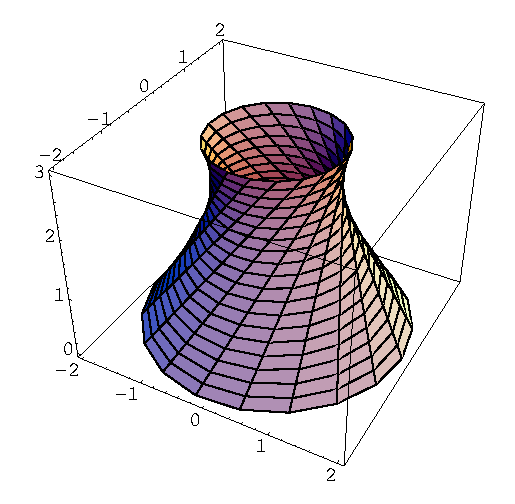
\epsfig{file=kuvat/hyperboloidi.eps}
\end{center}
\end{figure}
Pinnan kapein kohta on korkeudella $z=12/5$. \loppu

\pagebreak

\Harj
\begin{enumerate}

\item
Hahmottele seuraavien parametristen tasokäyrien kulku. Eliminoimalla parametri johda myös
käyrän yhtälö karteesisessa koordinaatistossa.
\begin{align*}
&\text{a)}\ \ x=2-t,\ y=t+1,\ t\in\R \qquad\ \text{b)}\ \ x=t^2,\ y=2-t,\ t\in[0,\infty) \\
&\text{c)}\ \ x=\frac{1}{t}\,,\ y=t-1,\ t\in(0,4) \qquad\,
 \text{d)}\ \ x=\frac{1}{1+t^2}\,,\ y=\frac{t}{1+t^2}\,,\ t\in\R \\
&\text{e)}\ \ \vec r=3\sin\pi t\,\vec i+4\cos\pi t\,\vec j,\ t\in[-1,1] \\[1mm]
&\text{f)}\ \ x=1-\sqrt{4-t^2}\,,\ y=2+t,\ t\in[-2,2] \\[1mm] 
&\text{g)}\ \ \vec r=t\cos t\,\vec i+t\sin t\,\vec j,\ t\in[0,4\pi]
\end{align*}

\item
a) Tasokäyrän eräs parametrisointi on $\vec r=\cos 2t\,\vec i+\sin^2 t\,\vec j,\ t\in\R$. 
Anna käyrälle vaihtoehtoinen, mahdollisimman yksinkertainen parametrisointi.
\vspace{1mm}\newline
b) Totea, että $\,\vec r=(t-1)\vec i+\sqrt{2t-t^2}\,\vec j,\ t\in[0,2]\,$ ja 
$\,\vec r=t\sqrt{2-t^2}\,\vec i+(1-t^2)\vec j$, \newline $t\in[-1,1]$ ovat saman käyrän 
parametrisointeja. Mikä käyrä on kyseessä?

\item \index{Cartesiuksen lehti}
Tasokäyrä $S:\,x^3+y^3=3xy\,$ on nimeltään \kor{Cartesiuksen lehti}. Johda käyrälle
parametriesitys kirjoittamalla $y=tx$. Hahmottele käyrän kulku parametrimuodosta ja merkitse
kuvioon, mitkä käyrän osat vastaavat parametrin arvoja väleillä $(-\infty,-1)$, $(-1,0)$ ja 
$[0,\infty)$. Miksei $t=-1$ vastaa mitään käyrän pistettä?

\item \index{venytetty sykloidi}
Ympyrä, jonka säde on $R=1$, vierii liukumatta pitkin positiivista $x$-akselia. Ympyrän mukana
pyörii siihen kiinnitetty jana, jonka toinen päätepiste on ympyrän keskipisteessä ja keskipiste
on ympyrän kehällä. Määritä janan toisen (ympyrän ulkopuolella olevan) päätepisteen sijainti
parametrisena käyränä $x=x(t),\ y=y(t)$, missä $t$ on ympyrän vierimiskulma mitattuna 
alkutilanteesta, jossa janan päätepisteet ovat $(0,1)$ ja $(0,3)$. Hahmottele käyrä
graafisesti. Missä pisteessä käyrä leikkaa ensimmäisen kerran itsensä? (Käyrää sanotaan 
\kor{venytetyksi sykloidiksi}.)

\item
Parametrisoi tason $T\,:x+y=4$ ja kartion $K:\,xy+yz+xz=0$ leikkauskäyrä ottamalla
parametriksi\, a) $t=x$, \ b) $t=x-y$.

\item
a) Avaruuskäyrän $S$ parametrisointi on $\vec r = \vec r_0+\cos t\,\vec a+\sin t\,\vec b$,
$\,t\in[0,2\pi]$, missä $\vec a$, $\vec b$ ja $\vec r_0$ ovat avaruusvektoreita. Täsmälleen
millä ehdoilla $S$ on avaruusympyrä?
\vspace{1mm}\newline
b) Avaruusympyrän keskipiste on $(1,1,2)$, säde on $R=3$ ja ympyrä on tasossa $x-y-3z+6=0$.
Johda ympyrälle jokin parametrisointi muotoa $\vec r=\vec r_0+\cos t\,\vec a+\sin t\,\vec b$,
$\,t\in[0,2\pi]$.

\item
Näytä, että yhtälöryhmä
$\D \ \begin{cases} \,x^2+y+z=2 \\ \,xy+z=1 \end{cases} $ \vspace{1mm}\newline
määrittelee kaksi leikkaavaa avaruuskäyrää, joista toisen parametrisointi on
$\vec r=t\vec i+(1+t)\vec j+(1-t-t^2)\vec k,\ t\in\R$. Millainen on toinen käyrä?

\item \index{zzb@\nim!Kiukkulintu ja kuulantyöntäjät} (Kiukkulintu ja kuulantyöntäjät)\, 
a) Kiukkulintu lennätetään alkupisteestä $(x,y)$ $=(0,1)$ (pituusyksikkö = cm) venyttämällä 
heittoparaabelissa (ks.\ Esimerkki\,\ref{heittoparaabeli}) vakion $a$ arvoksi $8$ cm ja
tähtäämällä porsaaseen, joka on pisteessä $(4,3)$. Millä $k$:n arvoilla tulee
osuma? \vspace{1mm}\newline 
b) Teekkarit Yrjölä ja Ståhlberg kisaavat kuulantyönnössä. Ratkaise, kumpi voitti, kun
kisaajien parhaissa työnnöissä heittoparaabelin parametrit ovat \newline
Yrjölä:   $\,\ \qquad h=2.00$ m, $\ \alpha=60.0\aste$, $\ a=8.00$ m \newline
Ståhlberg: $\quad h=1.80$ m, $\ \alpha=30.0\aste$, $\ a=6.65$ m

\item
Esitä jokin parametrisointi seuraavien yhtälöiden määräämille pinnoille: \newline
a)\, $x^3y^2z=5,\,\ $ b)\, $(x-z)(x+z)+y+2z=0,\,\ $ c)\, $x\sin z+xy^5+y=1$

\item
a) Johda pinnalle $S$ yhtälö muotoa $F(x,y,z)=0$ parametrisoinnista
\[ 
S:\ \begin{cases}
    \,x=3+2\sin\theta\cos\varphi, \\
    \,y\,=-1+\sin\theta\sin\varphi, \\
    \,z=2+3\cos\theta, \quad (\theta,\varphi)\in\Rkaksi.
    \end{cases}
\]
b) Pallon $K$ keskipiste on $(1,1,1)$ ja säde on $R=2$. Kuvan piirtoa varten halutaan
parametrisoida pallon $xy$-tason yläpuolinen ($z \ge 0$) osa. Esitä parametrisointi!
\vspace{1mm}\newline
c) Pinnan $S$ yhtälö lieriökoordinaateissa on $\,r=\varphi,\ (\varphi,z) \in A$, missä
$A=[0,4\pi]\times[-5,5]$. Parametrisoi $S$ viivoitinpintana. Millainen on $S$:n ja
$xy$-tason leikkauskäyrä? \vspace{1mm}\newline
d) Pinnan yhtälö lieriökoordinaateissa on $r=z^2\abs{\cos\varphi}$. Esitä pinnan yhtälö
karteesisissa koordinaateissa. Millaisia ovat pinnan ja tasojen $z=c$ ($c\in\R$)
leikkauskäyrät?

\item \index{hyperboloidi} \index{kaksivaippainen hyperboloidi}
a) Määritä sen viivoitinpinnan yhtälö (muodossa $F(x,y,z)=0$), joka syntyy, kun suora
$S:\ x=z,\ y=1$ pyörähtää $x$-akselin ympäri. Totea, että sama pinta (nimeltään yksivaippainen
hyperboloidi) syntyy myös, kun eräs $xy$-tason käyrä $K$ pyörähtää $x$-akselin ympäri. 
Hahmottele $K$ graafisesti. \vspace{1mm}\newline 
b) Tasokäyrän $K: x^2-y^2=1$ pyörähtäessä $x$-akselin ympäri syntyy pinta nimeltä
\kor{kaksivaippainen hyperboloidi}. Määritä ko.\ pinnan yhtälö. Missä pisteissä suora
$x=y=z$ leikkaa pinnan?

\item
a) Puolikartion $K$ kärki on origossa, symmetria-akseli on positiivinen $z$-akseli ja
puolisuora $x=2y=3z,\ x \ge 0$ on pinnalla $K$. Parametrisoi $K$ pyörähdyspintana ja
viivoitinpintana. Mikä on $K$:n yhtälö lieriökoordinaatistossa? \vspace{1mm}\newline
b) Parametrisoi kartio $K:\ xy+yz+xz=0\,$ viivoitinpintana.

\item (*) \index{asteroidi} \index{hyposykloidi}
Ympyrän keskipiste on origossa ja säde on $a$. Ympyrää pitkin sen sisäpuolella vierii liukumatta
toinen ympyrä, jonka säde on $b<a$. Tällöin vierivän ympyrän kiinteä piste $P$ piirtää 
tasokäyrän nimeltä \kor{hyposykloidi}. \ a) Näytä, että pisteen $(a,0)$ kautta kulkevan
hyposykloidin parametriesitys on
\[
x=(a-b)\cos t+b\cos\left(\frac{a-b}{b}\,t\right), \quad
y=(a-b)\sin t-b\sin\left(\frac{a-b}{b}\,t\right).
\]
b) Päättele, että tapauksessa $a=2b$ piste $P$ liikkuu pitkin janaa. \newline
c) Näytä, että tapauksessa $a=4b$ parametriesitys yksinkertaistuu muotoon 
\[
x=a\cos^3 t,\ \ y=a\sin^3 t.
\] 
Hahmottele tämän käyrän --- nimeltään \kor{asteroidi} --- kulku. Mikä on asteroidin yhtälö
karteesisissa koordinaateissa? 

\item (*) \index{zzb@\nim!Sotaharjoitus 1}
(Sotaharjoitus 1) Origosta ammutun tykinkuulan lentorata on ajan $t$ funktiona (yksiköt km ja s)
\[ \begin{cases}
x(t)=(\sin\theta\cos\varphi+a)\,t, \\
y(t)=(\sin\theta\sin\varphi+b)\,t, \\
z(t)=(\cos\theta)\,t-0.005\,t^2,
\end{cases} \]
missä $\theta,\varphi$ ovat suuntauskulmat ja $a,b$ ovat tuuliparametreja. Maastoesteet
asettavat suuntaukselle rajoituksen $\tan\theta > 0.2$. Miten suuntaus on valittava 
tuulettomassa säässä ($a=b=0$), jotta ammus osuisi pisteessä $(10,20,0)$ olevaan maaliin? 
Kuinka korkealla ammus käy? Kuinka kauas maalista ammus osuu tällä suuntauksella, jos 
$a=0.002$ ja $b=-0.001$\,? %Miten suuntausta olisi (likimain) muutettava?

\item (*)
Jana, jonka pituus on $20$, liikkuu seuraavasti: Janan keskipiste liikkuu $z$-akselia pitkin
positiiviseen suuntaan vakionopeudella. Liikkuessaan jana pysyy $xy$-tason suuntaisena ja pyörii
tasaisesti (kulmanopeus vakio) siten, että keskipisteen liikkuessa $30$ pituusyksikköä
jana pyörii täyden kierroksen positiivisen $z$-akselin suunnasta katsottuna vastapäivään.
Esitä janan avaruuteen piirtämän viivoitinpinnan $S$ parametrisointi, kun tiedetään lisäksi,
että piste $(1,0,0)$ on tällä pinnalla. Leikkaako suora $z=25,\ x+y=4$ pinnan $S$\,?

\end{enumerate}